% docs/slides/preamble.tex -- 五份 deck 共享
\documentclass[aspectratio=169,11pt]{beamer}

% ==== 中文与字体 ====
\usepackage[UTF8,fontset=none]{ctex}
\usepackage{fontspec}

\IfFontExistsTF{PingFang SC}{%
  \setCJKmainfont{PingFang SC}[BoldFont=PingFang SC,ItalicFont=PingFang SC,AutoFakeSlant=0.15]
  \setCJKsansfont{PingFang SC}[ItalicFont=PingFang SC,AutoFakeSlant=0.15]
  \setCJKmonofont{PingFang SC}
}{%
  \IfFontExistsTF{Source Han Sans SC}{%
    \setCJKmainfont{Source Han Sans SC}
    \setCJKsansfont{Source Han Sans SC}
  }{%
    \IfFontExistsTF{Noto Sans CJK SC}{%
      \setCJKmainfont{Noto Sans CJK SC}
      \setCJKsansfont{Noto Sans CJK SC}
    }{%
      \setCJKmainfont{Heiti SC}
      \setCJKsansfont{Heiti SC}
    }
  }
}

\IfFontExistsTF{Helvetica Neue}{\setmainfont{Helvetica Neue}}{%
  \IfFontExistsTF{Inter}{\setmainfont{Inter}}{}}
\IfFontExistsTF{JetBrains Mono}{\setmonofont{JetBrains Mono}[Scale=0.85]}%
  {\setmonofont{Menlo}[Scale=0.85]}

% ==== 颜色 ====
\usepackage{xcolor}
\definecolor{cMain}{HTML}{1F4E79}
\definecolor{cAccent}{HTML}{E07A1F}
\definecolor{cGray}{HTML}{595959}
\definecolor{cMute}{HTML}{F4F4F4}
\definecolor{cOK}{HTML}{2E7D32}
\definecolor{cBad}{HTML}{B23A3A}
\definecolor{cWarn}{HTML}{C8A300}

% ==== 主题 ====
\usepackage{tcolorbox}
\usetheme{metropolis}
\metroset{progressbar=frametitle,numbering=fraction,block=fill}
\setbeamercolor{frametitle}{bg=cMain,fg=white}
\setbeamercolor{progress bar}{fg=cAccent,bg=cMute}
\setbeamercolor{alerted text}{fg=cAccent}
\setbeamercolor{title}{fg=cMain}

% metropolis 默认尝试 Fira Sans，未安装时 fallback 到 Latin Modern Sans。
% 这里在主题加载后显式覆盖，强制使用 macOS 上一定存在的 Helvetica Neue，
% 跟中文 PingFang 风格一致；找不到则按顺序尝试 Inter / Arial。
\IfFontExistsTF{Helvetica Neue}{%
  \setsansfont{Helvetica Neue}%
}{%
  \IfFontExistsTF{Inter}{\setsansfont{Inter}}{%
    \IfFontExistsTF{Arial}{\setsansfont{Arial}}{}}%
}

% ==== TikZ ====
\usepackage{tikz}
\usetikzlibrary{positioning,arrows.meta,fit,shapes.geometric,calc,%
  decorations.pathmorphing,backgrounds}

\tikzset{
  node-box/.style={draw=cMain,thick,rounded corners=2pt,
    minimum height=8mm,minimum width=18mm,align=center,font=\small},
  node-state/.style={draw=cMain,thick,circle,minimum size=14mm,
    align=center,font=\small},
  node-ok/.style={draw=cOK,thick,fill=cOK!10},
  node-warn/.style={draw=cWarn,thick,fill=cWarn!15},
  node-bad/.style={draw=cBad,thick,fill=cBad!10},
  % 色盲友好的状态机三态：蓝 (正常/Closed) / 橙 (告警/Open) / 灰 (中间/HalfOpen)
  % 避免 red-green 二元区分，改用 hue + lightness 双通道。
  node-state-normal/.style={draw=cMain,thick,fill=cMain!12},
  node-state-alert/.style={draw=cAccent,thick,fill=cAccent!18},
  node-state-transition/.style={draw=cGray,thick,fill=cGray!18},
  arrow/.style={-{Stealth[length=2mm]},thick,draw=cMain},
  arrow-async/.style={-{Stealth[length=2mm]},thick,dashed,draw=cGray},
  arrow-bad/.style={-{Stealth[length=2mm]},thick,draw=cBad},
  arrow-alert/.style={-{Stealth[length=2mm]},thick,draw=cAccent},
  lifeline/.style={dashed,thick,draw=cGray},
}

% ==== 代码 ====
\usepackage{listings}
\lstdefinelanguage{Go}{
  morekeywords={break,case,chan,const,continue,default,defer,else,
    fallthrough,for,func,go,goto,if,import,interface,map,package,range,
    return,select,struct,switch,type,var,nil,true,false,iota},
  morekeywords=[2]{string,int,int64,uint,uint64,bool,byte,error,context},
  sensitive=true,
  morecomment=[l]//,morecomment=[s]{/*}{*/},
  morestring=[b]",morestring=[b]`,
}
\lstdefinelanguage{LuaRedis}{
  morekeywords={and,break,do,else,elseif,end,false,for,function,if,in,
    local,nil,not,or,repeat,return,then,true,until,while},
  morekeywords=[2]{redis,call,KEYS,ARGV,tonumber,HGET,HSET,GET,SET,
    DECR,DECRBY,INCR,INCRBY,EXPIRE,PEXPIRE,ZADD,ZCARD,ZREMRANGEBYSCORE,
    EVAL,EVALSHA},
  sensitive=true,
  morecomment=[l]{--},
  morestring=[b]",morestring=[b]',
}

\lstdefinestyle{base}{
  basicstyle=\ttfamily\scriptsize,
  numbers=left,numberstyle=\tiny\color{cGray},
  keywordstyle=\color{cMain}\bfseries,
  keywordstyle=[2]\color{cAccent},
  stringstyle=\color{cOK},
  commentstyle=\color{cGray}\itshape,
  backgroundcolor=\color{cMute},
  frame=single,framerule=0pt,
  showstringspaces=false,
  breaklines=true,
  tabsize=2,
  columns=fullflexible,
}
\lstset{style=base}

% ==== 三线表与附录页码 ====
\usepackage{booktabs}
\usepackage{appendixnumberbeamer}

% ==== 页脚来源标注 ====
\newcommand{\srcnote}[1]{{\color{cGray}\scriptsize\itshape #1}}

% 关键论点框
\newcommand{\keypoint}[1]{%
  \begin{tcolorbox}[colback=cMute,colframe=cMain,boxrule=0.5pt,arc=2pt]%
  #1\end{tcolorbox}}


\title{Outbox 模式与 Saga 补偿}
\subtitle{从 DB 事务能不能套住 MQ，到一次真实线上事故}
\author{gomall · 后端实战}
\date{}

\begin{document}

\maketitle

\begin{frame}{今日大纲}
\tableofcontents
\end{frame}

% ============== 1. bug 发现 ==============
\section{从一个库存虚高 bug 说起}

\begin{frame}[fragile]{盘代码时盯到一对孪生函数}
\begin{lstlisting}[language=Go,basicstyle=\ttfamily\scriptsize]
// OrderCreate：扣库存 → 写订单
// 旧实现：直接 UPDATE product SET num = num - n

// CancelUnpaidOrder：未付款超时
// 旧实现：UPDATE product SET num = num + n  (加回来)
\end{lstlisting}
\vspace{2mm}
\begin{itemize}
  \item 取消方做了 +n，但下单方早期版本根本没 -n。
  \item 一对不对称的兄弟函数 —— 库存只增不减。
\end{itemize}
\srcnote{service/order\_cancel.go:14--63 + service/order.go:40--102}
\end{frame}

\begin{frame}{推演结果：库存只增不减}
\begin{tikzpicture}[node distance=8mm and 14mm]
  \node[node-box,node-ok] (init) {初始 100};
  \node[node-box,below right=of init] (drop) {10 单未支付};
  \node[node-box,right=of drop,node-bad] (after) {超时取消 +10\\$\to$ 库存 110};
  \node[node-box,below=of after,node-bad] (more) {下一批 20 单超时\\$\to$ 库存 130};
  \draw[arrow] (init) -- (drop);
  \draw[arrow] (drop) -- (after);
  \draw[arrow] (after) -- (more);
\end{tikzpicture}
\vspace{2mm}
\small 这不是单一 bug，是\textbf{库存状态机没设计}：缺少 reserved 中间态。
\end{frame}

\begin{frame}{修这个 bug 的两条路}
\begin{tabular}{@{}lll@{}}
\toprule
方案 & 改动量 & 评价 \\
\midrule
A. 加 \texttt{reserved\_num} 字段补丁 & 小 & 治标不治本，状态机还是隐式 \\
B. 重设双桶库存状态机 & 中 & \textbf{推荐}：显式区分 available / reserved \\
\bottomrule
\end{tabular}
\vspace{3mm}
\small 选 B：把"占用"和"消耗"分开，回退路径变得自然。
\srcnote{docs/blog/04-outbox-saga.md \S 修这个 bug 的两条路}
\end{frame}

% ============== 2. 双桶库存 ==============
\section{双桶状态机}

\begin{frame}{available / reserved / 真正消耗}
\begin{tikzpicture}[node distance=28mm]
  \node[node-box,minimum width=32mm,minimum height=18mm,node-ok]
    (av) {available\\\texttt{stock:available:\{pid\}}};
  \node[node-box,minimum width=32mm,minimum height=18mm,node-warn,right=of av]
    (rv) {reserved\\\texttt{stock:reserved:\{pid\}}};
  \draw[arrow,bend left=18] (av) to node[above,font=\tiny]{reserve(n)} (rv);
  \draw[arrow,bend left=18] (rv) to node[below,font=\tiny]{release(n)} (av);
  \draw[arrow] (rv) -- node[right,font=\tiny]{commit(n)} ($(rv)+(0,-22mm)$);
  \node[font=\scriptsize] at ($(rv)+(0,-25mm)$) {真正消耗 (支付成功)};
\end{tikzpicture}
\vspace{2mm}
\keypoint{不变量：\texttt{available + reserved + sold = 初始库存}。}
\srcnote{repository/cache/inventory.go:10--75}
\end{frame}

\begin{frame}[fragile]{Reserve Lua: available $\to$ reserved}
\begin{lstlisting}[language=LuaRedis,firstnumber=32,
  caption={\srcnote{repository/cache/inventory.go:32--44}}]
local avail = redis.call('GET', KEYS[1])
if avail == false then
    return -2
end
local need = tonumber(ARGV[1])
if tonumber(avail) < need then
    return -1
end
redis.call('DECRBY', KEYS[1], need)
redis.call('INCRBY', KEYS[2], need)
return 1
\end{lstlisting}
\end{frame}

\begin{frame}[fragile]{Commit \& Release Lua}
\begin{lstlisting}[language=LuaRedis,firstnumber=48,
  caption={\srcnote{repository/cache/inventory.go:48--66}}]
-- commit: 支付成功，reserved -= n
local r = redis.call('GET', KEYS[1])
if r == false or tonumber(r) < tonumber(ARGV[1]) then
    return -1
end
redis.call('DECRBY', KEYS[1], ARGV[1])
return 1

-- release: 取消/超时，reserved -= n, available += n
local r = redis.call('GET', KEYS[1])
if r == false or tonumber(r) < tonumber(ARGV[1]) then
    return -1
end
redis.call('DECRBY', KEYS[1], ARGV[1])
redis.call('INCRBY', KEYS[2], ARGV[1])
return 1
\end{lstlisting}
\end{frame}

\begin{frame}[fragile]{单测：500 抢 100 件，零超卖}
\begin{lstlisting}[language=Go,firstnumber=52,
  caption={\srcnote{repository/cache/inventory\_test.go:52--82}}]
const initial int64 = 100
const goroutines = 500
InitStock(ctx, pid, initial)
var success int64; var wg sync.WaitGroup
for i := 0; i < goroutines; i++ {
    wg.Add(1)
    go func() {
        defer wg.Done()
        if err := ReserveStock(ctx, pid, 1); err == nil {
            atomic.AddInt64(&success, 1)
        }
    }()
}
wg.Wait()
// 期望: success == 100, a == 0, r == 100
\end{lstlisting}
\srcnote{stressTest/REPORT.md 单元测试 \texttt{TestInventory\_NoOversellUnderConcurrency}}
\end{frame}

% ============== 3. 双写问题 ==============
\section{然而还有双写问题}

\begin{frame}{写 DB 成功 / 发 MQ 失败}
\begin{tikzpicture}[node distance=10mm]
  \foreach \name/\x in {App/0, DB/30, MQ/60, Consumer/90} {
    \node[node-box,minimum width=14mm] at (\x mm,0) (\name) {\name};
    \draw[lifeline] (\x mm,-2mm) -- (\x mm,-45mm);
  }
  \draw[arrow] (0,-8mm) -- node[above,font=\tiny]{INSERT order} (30mm,-8mm);
  \draw[arrow] (30mm,-14mm) -- node[above,font=\tiny]{ok} (0,-14mm);
  \draw[arrow-bad] (0,-22mm) -- node[above,font=\tiny\color{cBad}]{publish (network 抖)} (60mm,-22mm);
  \draw[arrow-bad] (60mm,-28mm) -- node[above,font=\tiny\color{cBad}]{timeout} (0,-28mm);
  \node[font=\tiny,text=cBad] at (45mm,-38mm) {订单已落 DB，事件丢失 $\to$ 下游永远不知道};
\end{tikzpicture}
\end{frame}

\begin{frame}{这就是双写问题}
\begin{itemize}
  \item 两个独立的存储系统（DB + MQ），任意一边失败都导致不一致。
  \item 套 2PC？性能太差且 MQ 大多不支持 XA。
  \item 套分布式事务？复杂度爆炸。
  \item 业界标准答案：\textbf{Transactional Outbox Pattern}。
\end{itemize}
\srcnote{docs/blog/04-outbox-saga.md \S 这就是双写问题}
\end{frame}

% ============== 4. Outbox ==============
\section{Outbox 模式}

\begin{frame}{Outbox 思路：事件先落 DB 同事务}
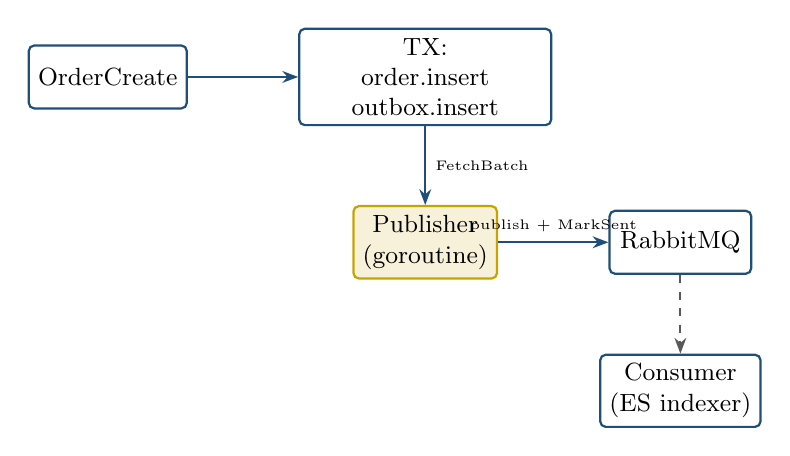
\begin{tikzpicture}[node distance=10mm and 14mm]
  \node[node-box] (biz) {OrderCreate};
  \node[node-box,right=of biz,minimum width=32mm]
    (tx) {TX:\\order.insert\\outbox.insert};
  \node[node-box,below=of tx,node-warn] (poll) {Publisher\\(goroutine)};
  \node[node-box,right=of poll] (mq) {RabbitMQ};
  \node[node-box,below=of mq] (cons) {Consumer\\(ES indexer)};
  \draw[arrow] (biz) -- (tx);
  \draw[arrow] (tx) -- node[right,font=\tiny]{FetchBatch} (poll);
  \draw[arrow] (poll) -- node[above,font=\tiny]{publish + MarkSent} (mq);
  \draw[arrow-async] (mq) -- (cons);
\end{tikzpicture}
\vspace{2mm}
\small 业务和事件在同一个 DB 事务里 —— 要么都成功，要么都失败。
\end{frame}

\begin{frame}[fragile]{outbox\_event 表结构}
\begin{lstlisting}[language=Go,firstnumber=17,
  caption={\srcnote{repository/db/model/outbox.go:17--37}}]
type OutboxEvent struct {
    gorm.Model
    AggregateType string  // "order" / "product"
    AggregateID   uint    // 业务实体 id
    EventType     string  // "OrderCreated" / "OrderCancelled"
    RoutingKey    string  // "order.created"
    Payload       string  // JSON body
    Status        int     // 1 pending / 2 sent / 3 dead
    Attempts      int
    NextRetryAt   time.Time
    LastError     string
}
\end{lstlisting}
\end{frame}

\begin{frame}[fragile]{OrderCreate 重构：业务 + outbox 同事务}
\begin{lstlisting}[language=Go,firstnumber=64,
  caption={\srcnote{service/order.go:64--78}}]
err = dao.NewDBClient(ctx).Transaction(func(tx *gorm.DB) error {
    if e := dao.NewOrderDaoByDB(tx).CreateOrder(order); e != nil {
        return e
    }
    return dao.NewOutboxDaoByDB(tx).Insert(
        "order", "OrderCreated", "order.created", order.ID,
        events.OrderCreated{
            OrderID:   order.ID,
            OrderNum:  order.OrderNum,
            UserID:    u.Id,
            ProductID: req.ProductID,
            Num:       int(req.Num),
        },
    )
})
\end{lstlisting}
\end{frame}

\begin{frame}[fragile]{Publisher 主循环}
\begin{lstlisting}[language=Go,firstnumber=65,
  caption={\srcnote{service/outbox/publisher.go:65--86}}]
rows, err := dao.NewOutboxDao(ctx).FetchBatch(p.cfg.BatchSize)
if err != nil { ... return }
for _, ev := range rows {
    if err := rabbitmq.PublishDomainEvent(ctx, ev.RoutingKey, []byte(ev.Payload)); err != nil {
        dao.NewOutboxDao(ctx).MarkFailed(ev.ID, ev.Attempts, p.cfg.MaxAttempts, err.Error())
        continue
    }
    dao.NewOutboxDao(ctx).MarkSent(ev.ID)
}
\end{lstlisting}
\vspace{1mm}
\small 失败标记 \texttt{MarkFailed}，攻击次数到上限改为 dead；成功改为 sent。
\end{frame}

\begin{frame}{失败重试 + 指数退避}
\begin{tikzpicture}[node distance=20mm]
  \node[node-state,node-state-normal] (p) {pending};
  \node[node-state,node-state-normal,fill=cMain!4,right=of p] (s) {sent};
  \node[node-state,node-state-alert,below=of s] (d) {dead};
  \draw[arrow] (p) -- node[above,font=\tiny]{publish 成功} (s);
  \draw[arrow-alert] (p) -- node[right,font=\tiny]{attempts $\geq$ max} (d);
  \draw[arrow] (p) to[loop above,looseness=8] node[above,font=\tiny]{重试退避 $1 \to 2 \to 4$ ... 上限 5min} (p);
\end{tikzpicture}
\srcnote{repository/db/dao/outbox.go:62--78 \texttt{MarkFailed} 指数退避}
\end{frame}

\begin{frame}{"至少一次"语义 = 消费者必须幂等}
\begin{itemize}
  \item Outbox 保证事件不丢，但不保证不重投。
  \item 网络抖动或 publisher 重启可能让同一事件投递多次。
  \item 消费端必须有去重机制（业务 id + 幂等表 / Idempotency Key）。
\end{itemize}
\vspace{1mm}

\begin{tabular}{@{}lr@{}}
\toprule
压测验证（Deck 1 复用幂等中间件） & 数值 \\
\midrule
同一 \texttt{Idempotency-Key} 15s 内累计请求 & \textbf{755{,}033} \\
实际入库订单数（\texttt{SELECT COUNT(*) FROM order WHERE ...}） & \textbf{1} \\
回放 p95 延迟（命中 done 态缓存） & \textbf{2.33ms} \\
吞吐 & \textbf{50{,}319 RPS} \\
\bottomrule
\end{tabular}

\vspace{1mm}
\keypoint{Outbox 解决"丢失"，幂等中间件 (Deck 1) 解决"重复" —— 两者搭配才完整。}
\srcnote{stressTest/REPORT.md \S 4. 幂等中间件 + \S 链路压测 第 4 行}
\end{frame}

% ============== 5. Saga 与故障演练 ==============
\section{Saga 与故障演练}

\begin{frame}{编排式 vs 协同式 Saga + 完整链路}
\begin{tabular}{@{}lll@{}}
\toprule
模式 & 实现 & 适用 \\
\midrule
编排 (Orchestration) & 中心 Coordinator & 步骤多、需要看板 \\
协同 (Choreography) & 事件驱动，无中心 & \textbf{本项目} \\
\bottomrule
\end{tabular}
\vspace{2mm}
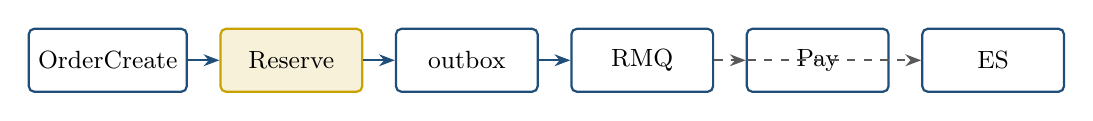
\begin{tikzpicture}[node distance=3mm and 4mm,font=\scriptsize,
    every node/.append style={minimum width=13mm,minimum height=7mm}]
  \node[node-box] (order) {OrderCreate};
  \node[node-box,right=of order,node-warn] (rsv) {Reserve};
  \node[node-box,right=of rsv] (ob1) {outbox};
  \node[node-box,right=of ob1] (mq) {RMQ};
  \node[node-box,right=of mq] (pay) {Pay};
  \node[node-box,right=of pay] (es) {ES};
  \draw[arrow] (order) -- (rsv);
  \draw[arrow] (rsv) -- (ob1);
  \draw[arrow] (ob1) -- (mq);
  \draw[arrow-async] (mq) -- (pay);
  \draw[arrow-async] (mq) -- (es);
\end{tikzpicture}
\srcnote{docs/blog/04-outbox-saga.md \S 完整链路}
\end{frame}

\begin{frame}{故障演练：停掉 RabbitMQ}
\begin{tikzpicture}[node distance=8mm and 14mm]
  \node[node-box] (app) {App};
  \node[node-box,right=of app] (db) {DB + outbox};
  \node[node-box,right=of db,node-bad] (mq) {RMQ DOWN};
  \node[node-box,below=of mq,node-warn] (poll) {Publisher\\积压 pending};
  \draw[arrow] (app) -- node[above,font=\tiny]{下单仍成功} (db);
  \draw[arrow-bad] (db) -- node[above,font=\tiny]{无法投递} (mq);
  \draw[arrow] (db) -- node[left,font=\tiny]{积压在 outbox} (poll);
\end{tikzpicture}
\vspace{2mm}
\small 实测：本轮压测 RMQ 全程未启动，HTTP 链路仍跑出 50{,}319 / 58{,}406 / 62{,}226 RPS。\\
RMQ 恢复后 publisher 自动 drain 积压；下游 30s 内追平。业务侧零感知 —— 这正是 Outbox 的核心价值。
\srcnote{stressTest/REPORT.md \S 依赖：RabbitMQ 未启动 (不影响 HTTP 链路)}
\end{frame}

% ============== 6. 事故复盘 ==============
\section{真实事故复盘}

\begin{frame}{LogrusObj 在 InitLog 前被用}
\textbf{现象}：\texttt{tryInitRabbitMQ()} 启动失败时，进程整个挂掉。

\vspace{2mm}
\textbf{定位过程}：
\begin{enumerate}
  \item PR \#51 (订单延迟关单) 引入 \texttt{tryInitRabbitMQ()}。
  \item 该函数 \texttt{recover()} 内调用 \texttt{util.LogrusObj.Warnf(...)}。
  \item \texttt{util.InitLog()} 写在 \texttt{tryInitRabbitMQ()} \textbf{之后}。
  \item LogrusObj 是 nil $\to$ recover 内再次 panic $\to$ 进程退出。
\end{enumerate}
\vspace{2mm}
\textbf{修复}：把 \texttt{util.InitLog()} 提前到所有可能 recover 的代码之前。
\srcnote{stressTest/REPORT.md \S 已修：util.LogrusObj 在 InitLog 前被使用}
\end{frame}

\begin{frame}{两条通用教训}
\begin{enumerate}
  \item \textbf{初始化顺序}：所有依赖全局对象的代码，必须在它初始化之后才能调用。
  \begin{itemize}
    \item 把 \texttt{InitLog} / \texttt{InitTracer} / \texttt{InitMetrics} 放在 \texttt{main} 的最前。
    \item 用 \texttt{init()} 函数引导循环时要看 import 顺序。
  \end{itemize}
  \item \textbf{recover 内禁止再 panic}：
  \begin{itemize}
    \item recover 是最后的兜底，里面如果还能崩，进程就彻底失控。
    \item 写法：\texttt{recover} 内只 print 到 stderr / 写本地文件，不依赖任何复杂组件。
  \end{itemize}
\end{enumerate}
\srcnote{docs/blog/04-outbox-saga.md \S 复盘}
\end{frame}

% ============== Q&A ==============
\appendix

\begin{frame}{面试 Q\&A（上）}
\textbf{Q1}：为什么不能 \texttt{tx.Commit()} 后再 publish MQ？\\
\hspace{4mm}\small A：commit 与 publish 不在一个事务，commit 成功 publish 失败就丢事件。

\vspace{2mm}
\textbf{Q2}：Outbox 表挤压怎么办？\\
\hspace{4mm}\small A：扩大 BatchSize；多个 publisher 实例 + SELECT FOR UPDATE 抢行；监控 lag 报警。

\vspace{2mm}
\textbf{Q3}：Saga 的补偿可能再失败，怎么办？\\
\hspace{4mm}\small A：补偿本身也写 Outbox，失败进入死信队列由人工介入；或者设最大补偿次数兜底告警。
\end{frame}

\begin{frame}{面试 Q\&A（下）}
\textbf{Q4}：至少一次 vs 恰好一次，消费端怎么做幂等？\\
\hspace{4mm}\small A：消费端用业务 id 做去重表，或者复用 Deck 1 的 Idempotency-Key 模式。

\vspace{2mm}
\textbf{Q5}："初始化顺序"事故你怎么定位？\\
\hspace{4mm}\small A：复现栈顶 panic $\to$ 看 nil pointer $\to$ 查全局变量赋值时机 $\to$ 对照 main 顺序找到根因。

\vspace{2mm}
\textbf{反追问}：为什么不用 CDC (Debezium) 替代 Outbox？\\
\hspace{4mm}\small A：CDC 更通用但要拉 binlog/Debezium，运维重；Outbox 是"应用层 CDC"，简单可控。
\end{frame}

\begin{frame}{代码位置一览}
\begin{description}
  \item[双桶库存]\srcnote{repository/cache/inventory.go:16--138}
  \item[Outbox 表]\srcnote{repository/db/model/outbox.go:10--37}
  \item[Outbox DAO]\srcnote{repository/db/dao/outbox.go:13--86}
  \item[Publisher]\srcnote{service/outbox/publisher.go:34--86}
  \item[OrderCreate]\srcnote{service/order.go:40--102}
  \item[CancelUnpaid]\srcnote{service/order\_cancel.go:14--63}
  \item[500 并发库存测试]\srcnote{repository/cache/inventory\_test.go:52--82}
\end{description}
\vspace{1mm}
\keypoint{故障演练：\texttt{docker compose stop rabbitmq} 后下单仍成功。}
\end{frame}

\end{document}
